\graphicspath{{1contrev/asy/}}

\title{Math 140B - Notes}
\author{Neil Donaldson}
\date{\today}
\maketitle

\thispagestyle{empty}

\section{Continuity}

The overarching goal of this course and its prequel is to make elementary calculus rigorous. We begin with a review of some basic concepts and conventions.


\boldinline{Sets \& Functions}

In these notes, essentially all functions have the form $f:U\to V$ where both $U,V$ are subsets of the real numbers $\R$. To $f$ are associated several concepts:
\begin{description}\itemsep2pt
	\item[\normalfont\emph{Domain}] $\dom(f)=U$; the \emph{inputs} to $f$. Often \emph{implied} to be the largest set on which a formula is defined. In calculus examples, the domain is typically a union of (open) intervals.
	\item[\normalfont\emph{Codomain}] $\operatorname{codom}(f)=V$; the \emph{potential outputs} of $f$. By convention, $V=\R$ unless necessary.
	\item[\normalfont\emph{Range}] $\range(f)=f(U)=\{f(x):x\in U\}$; the \emph{realized outputs} of $f$ and a subset of $V$.
	\item[\normalfont\emph{Injectivity}] $f$ is \emph{injective/one-to-one} if $f(x)=f(y)\implies x=y$: distinct inputs produce distinct outputs.
	\item[\normalfont\emph{Surjectivity}] $f$ is \emph{surjective/onto} if $f(U)=V$: all potential outputs are realized.
	\item[\normalfont\emph{Inverses}] $f$ is \emph{bijective/invertible} if it is injective and surjective. Equivalently, $\exists f^{-1}:V\to U$ satisfying
	\[
		\forall u\in U,\ f^{-1}\bigl(f(u)\bigr)=u\quad\text{and}\quad \forall v\in V,\ f\bigl(f^{-1}(v)\bigr)=v
	\]
\end{description}

\begin{example}[lower separated=false, sidebyside, sidebyside align=top seam, sidebyside gap=0pt, righthand width=0.32\linewidth]{}{}
	The function defined by \smash{$f(x)=\frac 1{x(x-2)}$}
	has implied
	\begin{gather*}
		\textcolor{Green}{\dom(f)}=\R\setminus\{0,2\}=(-\infty,0)\cup(0,2)\cup (2,\infty)\\[5pt]
		\textcolor{Brown}{\range(f)}=(-\infty,-1]\cup(0,\infty)
	\end{gather*}
	The function is neither injective nor surjective.	By \textcolor{orange}{restricting} the domain \& codomain, we obtain a bijection:
	\begin{gather*}
		\textcolor{Green}{\dom(\hat f)}=[1,2)\cup(2,\infty)\\
		\textcolor{Brown}{\operatorname{codom}(\hat f)}=(-\infty,-1]\cup(0,\infty)\\
		\intertext{with inverse}
		\hat f^{-1}(y)=
		\begin{cases}
			1+y^{-1}\sqrt{y+1}&\text{if }y>0\\
			1-y^{-1}\sqrt{y+1}&\text{if }y\le -1
		\end{cases}
	\end{gather*}
	Now $\textcolor{Brown}{\dom(\hat f^{-1})}=\textcolor{Green}{\operatorname{codom}(\hat f)}$ and $\textcolor{Green}{\operatorname{codom}(\hat f^{-1})}=\textcolor{Brown}{\dom(\hat f)}$.
	\tcblower
	\flushright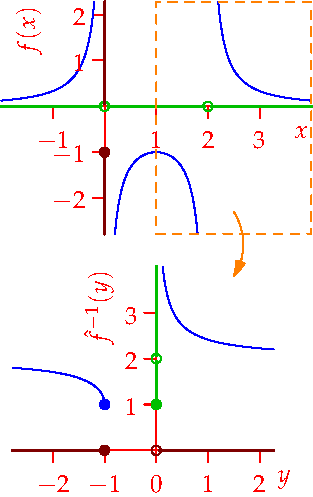
\includegraphics{dom4}
\end{example}

\goodbreak


\boldinline{Suprema and Infima}

A set $U\subseteq\R$ is \emph{bounded above} if it has an \emph{upper bound} $M$:
\[
	\exists M\in\R\text{ such that }\forall u\in U,\ u\le M
\]


\begin{axiom}{Completeness}{}
	If $U\subseteq\R$ is non-empty and bounded above, then it has a \emph{least upper bound,} the \emph{supremum} of $U$
	\[
		\sup U=\min\bigl\{M\in\R:\forall u\in U,\ u\le M\bigr\}
	\]
\end{axiom}

By convention, $\sup U:=\infty$ if $U$ is unbounded above and $\sup\emptyset:=-\infty$; now every subset of $\R$ has a supremum. Similarly, the \emph{infimum} of $U$ is its \emph{greatest lower bound}:
	\[
		\inf U=
		\begin{cases}
			\max\bigl\{m\in\R:\forall u\in U,\ u\ge m\bigr\} &\text{if $U\neq\emptyset$ is bounded below}\\
			-\infty&\text{if $U\neq\emptyset$ is unbounded below}\\
			\infty&\text{if $U=\emptyset$}
		\end{cases}
	\]
	
\begin{examples}{}{}
	Here are four sets with their suprema and infima stated. You should be able to verify these assertions directly from the definitions.
	\[
		\begin{array}{c||c|c|c|c|c}
			U&\{1,2,3,4\}&(0,5)&(-\infty,\pi]&\R&\{\frac 1n:n\in\N\}\\[2pt]\hline
			\sup U&4&5&\pi&\infty&1\\
			\inf U&1&0&-\infty&-\infty&0
		\end{array}
	\]
	Note how the supremum/infimum might or might not lie in the set itself.
\end{examples}


\boldinline{Interiors, closures, boundaries and neighborhoods}

These last concepts might not be review, but they will be used repeatedly.

\begin{defn}{}{interior}
	Let $U\subseteq\R$. A value $a\in\R$ is \emph{interior} to $U$ if it lies in some open subinterval of $U$:
	\[
		\exists\delta>0\text{ such that }(a-\delta,a+\delta)\subseteq U
	\]
	A \emph{neighborhood} of $a$ is any set to which $a$ is interior: the interval $(a-\delta,a+\delta)$ is an \emph{open $\delta$-neighborhood} of $a$. A \emph{punctured neighborhood} of $a$ is a neighborhood with $a$ deleted.\smallbreak
	The set of points interior to $U$ is denoted $U^\circ$.\smallbreak
	A \emph{limit point} of $U$ is the limit of some sequence $(x_n)\subseteq U$. The \emph{closure} $\cl U$ is the set of limit points.\smallbreak
	The \emph{boundary} of $U$ is the set $\partial U=\cl U\setminus U^\circ$.
\end{defn}

\begin{examples}{}{}
	\exstart If $U=[1,3)$, then $U^\circ=(1,3)$, \ $\cl U=[1,3]$ and $\partial U=\{1,3\}$.
	\begin{enumerate}\setcounter{enumi}{1}
	  \item $\Q^\circ=\emptyset$ and $\partial\Q=\cl\Q=\R$.
	  \item $(-3,5)\cup (5,7]$ is a punctured neighborhood of 5.
	\end{enumerate}
\end{examples}


\goodbreak
\clearpage


\setcounter{subsection}{16}
\subsection{Continuity of Functions}\label{sec:cont}

Everything in this section \emph{should} be review.

\begin{defn}{}{cont}
	A function $f:U\to\R$ is \emph{continuous at $u\in U$} if either/both of the following hold:
	\begin{enumerate}
	  \item For all sequences $(x_n)\subseteq U$ converging to $u$, the sequence $(f(x_n))$ converges to $f(u)$.
	  \item $\forall\epsilon>0$, $\exists\delta>0$ such that $(\forall x\in U)$, $\nm{x-u}<\delta\implies\nm{f(x)-f(u)}<\epsilon$.
	\end{enumerate}
	A function $f$ is \emph{continuous on $U$} if it is continuous at every point $u\in U$.
\end{defn}


\begin{examples}{}{}
	\exstart We prove that $f(x)=x^3$ is continuous at $u=2$.
	\begin{enumerate}\setcounter{enumi}{1}
		\item[]\begin{enumerate}
	  	\item (Limit method)\quad Let $x_n\to 2$. By the \emph{limit laws} (i.e. $\lim(x_n^k)=\left(\lim x_n\right)^k$),
			\[
				\lim_{x_n\to 2}f(x_n)=\lim_{x_n\to 2}x_n^3=\smash{\Bigl(\lim_{x_n\to 2}x_n\Bigr)^3}=2^3=f(2)
			\]
	  	\item ($\epsilon$--$\delta$ method)\quad Let $\epsilon>0$ be given and let $\displaystyle\delta=\smash{\min\left(1,\frac{\epsilon}{19}\right)}$.
			\[
				\nm{x-2}<\delta\implies \nm{x-2}<1\implies 1<x<3
			\]
			from which
			\[
				\nm{x^3-2^3}		
				=\nm{x-2}\nm{x^2+2x+2^2}
				<19\nm{x-2}\le\epsilon
			\]
			where we used the triangle inequality.
		\end{enumerate}
	
		\begin{minipage}[t]{0.70\linewidth}\vspace{0pt}
			\item Let $g(x)=
			\begin{cases}
				x\sin\frac 1x&\text{if }x\neq 0,\\
				0&\text{if }x=0
			\end{cases}$
			\smallbreak
			Then $g$ is continuous at $x=0$. Again this can be done with limits or an $\epsilon$--$\delta$ argument; both are essentially the \emph{squeeze theorem.}
	  
	  	\item The function defined by
	  	\[
	  		h(x)=
	  		\begin{cases}
	  		1+2x^2&\text{if }x<1\\
	  		2-x&\text{if }x\ge 1
	  		\end{cases}
	  	\]
	  	is discontinuous at $x=1$.
	  	\begin{enumerate}
	  		\item The sequence with $x_n=1-\frac 1n$ converges to 1, yet
				\[
					\lim h(x_n)=3\neq 1=h(1)
				\]
	   		\item Choose $\epsilon=1$ and suppose $\delta>0$ is given. Now choose $x=\max\{1-\frac\delta 2,\frac 1{\sqrt 2}\}$ to see that
				\[
					\nm{x-1}<\delta
					\quad\text{and}\quad 
					\nm{h(x)-h(1)}\ge 1=\epsilon
				\]
			\end{enumerate}
		\end{minipage}
		\hfill
		\begin{minipage}[t]{0.29\linewidth}\vspace{0pt}
			\flushright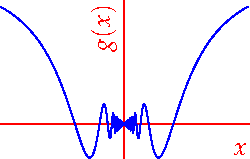
\includegraphics{cont-ex1}\bigbreak
			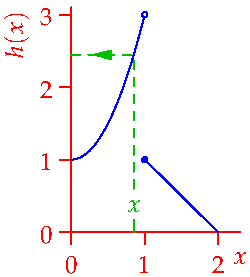
\includegraphics{cont-ex2}
		\end{minipage}
	
	
		
	% 	\begin{minipage}[t]{0.65\linewidth}\vspace{0pt}
	% 		\item We use both definitions to see that the function defined by
	%   \[h(x)=\begin{cases}
	%   1+2x^2&\text{if }x<1\\
	%   2-x&\text{if }x\ge 1
	%   \end{cases}\]
	%   is discontinuous at $x=1$.
	%   \begin{enumerate}
	%   	\item The sequence with $x_n=1-\frac 1n$ converges to 1, yet
	% 		\[\lim h(x_n)=3\neq 1=h(1)\]
	% %   	\item Choose $\epsilon=1$ and suppose $\delta>0$ is given. Choose any $x=\max\{1-\frac\delta 2,\frac 1{\sqrt 2}\}$ and observe that
	% %   	\[\nm{x-1}<\delta\quad\text{and}\quad \nm{h(x)-h(1)}\ge 1=\epsilon\]
	% 	\end{enumerate}
	% 	\end{minipage}\begin{minipage}[t]{0.35\linewidth}\vspace{0pt}
	% 	\flushright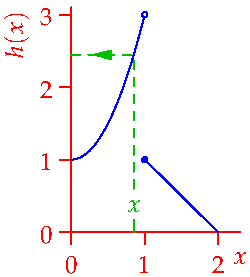
\includegraphics{cont-ex2}
	% 	\end{minipage}
	
	% 	\begin{enumerate}\setcounter{enumii}{1}
	% %   	\item The sequence with $x_n=1-\frac 1n$ converges to 1, yet
	% % 		\[\lim h(x_n)=3\neq 1=h(1)\]
	%   	\item Choose $\epsilon=1$, suppose $\delta>0$ is given, and let $x=\max\{1-\frac\delta 2,\frac 1{\sqrt 2}\}$ to observe that
	%   	\[\nm{x-1}<\delta\quad\text{and}\quad \nm{h(x)-h(1)}\ge 1=\epsilon\]
	% 	\end{enumerate}
	
	\end{enumerate} 
\end{examples}

\vfil\goodbreak


\begin{thm}{}{contdefequiv}
	The two parts of Definition \ref{defn:cont} are equivalent.
\end{thm}

\begin{proof}
	\begin{description}
		\item[\normalfont ($1\Rightarrow 2$)] We prove the contrapositive. Suppose condition 2 is \emph{false}; that is,
		\[
			\exists\epsilon>0,\text{ such that } 
			\forall\delta>0,\ \exists x\in U\text{ with } 
			\nm{x-u}<\delta\text{ and }
			\nm{f(x)-f(u)}\ge\epsilon
		\]
		In particular, for any $n\in\N$ we may let $\delta=\frac 1n$ to obtain
		\[
			\smash{\exists\epsilon>0,\text{ such that } 
			\forall n\in\N,\ \exists x_n\in U\text{ with }
			\nm{x_n-u}<\frac 1n\text{ and }
			\nm{f(x_n)-f(u)}\ge\epsilon}
		\]
		The sequence $(x_n)$ shows that condition 1 is \emph{false}:
		\begin{itemize}
	  	\item $\forall n, \ \nm{x_n-u}<\frac 1n$ whence $x_n\to u$.
	  	\item $\forall n, \ \nm{f(x_n)-f(u)}\ge\epsilon>0$, whence $f(x_n)$ \emph{does not converge to} $f(u)$.
		\end{itemize}
		
		\item[\normalfont ($2\Rightarrow 1$)] Suppose condition 2 is true, that $(x_n)\subseteq U$ converges to $u$ and that $\epsilon>0$ is given. Then
		\[
			\exists\delta>0\text{ such that }
			\nm{x-u}<\delta
			\implies \nm{f(x)-f(u)}<\epsilon
		\]
		However, by the definition of convergence ($x_n\to u$),
		\[
			\exists N\in\N \text{ such that }n>N
			\implies \nm{x_n-u}<\delta 
			\implies \nm{f(x_n)-f(u)}<\epsilon
		\]
		Otherwise said, $f(x_n)\to f(u)$.\qedhere
	\end{description}
\end{proof}

Rather than use these definitions every time, it is helpful to have a working dictionary.

\begin{thm}{Dictionary of Common Continuous Functions}{commoncont}
	\begin{enumerate}\setcounter{enumi}{0}\itemsep0pt
	  \item Suppose $f$ and $g$ are continuous at $u$ and that $k$ is constant. Then the following are continuous at $u$ (if defined---don't divide by zero!):
		\[
			f+g,\quad f-g,\quad fg,\quad \frac fg,\quad \nm f,\quad kf,\quad \max(f,g),\quad \min(f,g)
		\]
		\item If $f$ is continuous at $u$ and $h$ is continuous at $f(u)$, then $h\circ f$ is continuous at $u$.
	  \item Algebraic functions are continuous: these are functions constructed using finitely many addition/subtraction, multiplication/division and $n^\text{th}$ root operations.
		\item The familiar transcendental functions are continuous: $\exp$, $\ln$, $\sin$, etc.
	\end{enumerate}
\end{thm}


\begin{example}{}{}
	$f(x)=\sin\frac{\sqrt[3]{x^2+7}}{x-2}+\cos\frac 1{e^x-1}$ is continuous on its domain $(-\infty,0)\cup(0,1)\cup(1,\infty)$.
\end{example}


Theses claims are tedious to prove using elementary definitions. In particular, it is better to defer a proof of the transcendental claim until we can define such functions using power series, after which continuity comes for free.


\vfil\goodbreak

\begin{exercises}
	\emph{Key concepts/results:\quad Suprema/Completeness,\quad Sequential \& $\epsilon$-$\delta$ continuity}


% 	\exstart Give examples to show that $g\circ f$ being continuous can happen with:\vspace{-5pt}
	\begin{enumerate}\itemsep0pt%\setcounter{enumi}{1}  
	  \item Give examples to show that $g\circ f$ being continuous can happen with:
	  \begin{enumerate}
	    \item $f$ continuous and $g$ discontinuous. \qquad\qquad (b) \ $g$ continuous and $f$ discontinuous.
	    \item[(c)] Both $f,g$ discontinuous.
	  \end{enumerate}
	  You may use pictures, but make sure they clearly describe the functions $f,g$.
	  
	  
	  \item\begin{enumerate}
	  	\item Prove that the function $f(x)=x^3$ is continuous at $x=-2$ using an $\epsilon$--$\delta$ argument.
	  	\item Prove that $f(x)=x^3$ is continuous at $x=u$ using an $\epsilon$--$\delta$ argument.
	  \end{enumerate}
	
	
		\item Prove that the following are discontinuous at $x=0$: use \emph{both} definitions of continuity.
		\begin{enumerate}
	  	\item $f(x)=1$ for $x<0$ and $f(x)=0$ for $x\ge 0$.
	  	\item $g(x)=\sin(1/x)$ for $x\neq 0$ and $g(0)=0$.
		\end{enumerate}
		
		
		\item If $f$ is continuous at $u$, prove that it is bounded on some set $(u-\delta,u+\delta)\cap \dom(f)$.
	
	
		\item Prove the following parts of Theorem \ref{thm:commoncont} using $\epsilon$--$\delta$ arguments.
		\begin{enumerate}
	  	\item If $f,g$ are continuous at $u$, then $f-g$ is continuous at $u$.
	  	\item If $f,g$ are continuous at $u$, then $fg$ is continuous at $u$.
	  	\item If $f$ is continuous at $u$ and $h$ at $f(u)$, then $h\circ f$ is continuous at $u$.
		\end{enumerate}
	  
	  
	  \item\label{exs:isolatedcont} Suppose $f:U\to \R$ is a function whose domain $U$ contains an \emph{isolated point} $a$: i.e.\ $\exists r>0$ such that $(a-r,a+r)\cap U=\{a\}$. Prove that $f$ is continuous at $a$.
	  
	  
	  \item\label{exs:extremevaluelemma} Refresh your prerequisites by giving formal proofs:
	  \begin{enumerate}
	    \item (Suprema and sequences)\lstsp If $M=\sup U$, then $\exists (x_n)\subseteq U$ such that $x_n\to M$.\par
	    (\emph{This has to work even if $M=\infty$!})
	    \item (Limit of a bounded sequence)\lstsp If $(x_n)\subseteq[a,b]$ and $x_n\to x$, then $x\in [a,b]$.
			\item (Bolzano--Weierstraß)\lstsp Every bounded sequence in $\R$ has a convergent subsequence.\par
			(\emph{Hint: If $(x_n)\subseteq [a,b]$, explain why there exist intervals $I_1\supseteq I_2\supseteq I_3\supseteq\cdots$ such that \emph{infinitely many} $(x_n)$ lie in each interval $I_k$. Hence obtain a subsequence $(x_{n_k})$ and prove that it is \emph{Cauchy.}\footnotemark})
		\end{enumerate}
		
		
		\item (Hard)\lstsp Consider the function $f:\R\to\R$ where
		\[
			f(x)=
			\begin{cases}
				\frac 1q&\text{whenever }x=\frac pq\in\Q\text{ with }q>0\text{ and }\gcd(p,q)=1\\
				0&\text{ if }x\not\in\Q
			\end{cases}
		\]
	  For example, $f(1)=f(2)=f(-7)=1$, and $f(\tfrac 12)=f(-\tfrac 12)=f(\tfrac 32)=\cdots=\frac 12$, etc. Prove that $f$ is continuous at each point of $\R\setminus\Q$ and discontinuous at each point of $\Q$.
	\end{enumerate}
\end{exercises}

%\vspace{-10pt}

\footnotetext{%
	This is a good moment to review the notion of a Cauchy sequence
	\[
		\forall \epsilon>0,\exists N$ such that $m,n>N
		\implies \nm{x_m-x_n}<\epsilon
	\]
	and the discussion of Cauchy completeness: $(x_n)\subseteq\R$ is convergent if and only if it is Cauchy.%
}


\goodbreak



\subsection{Properties of Continuous Functions}\label{sec:propcont}


In this section we describe the behavior of a continuous function on an interval. We first consider the special case when the domain is a closed bounded interval $[a,b]$.

% \begin{defn}{}{}
% A function $f:U\to V$ is \emph{bounded} if $\exists M\in\R$ such that $\forall x\in U,\ \nm{f(x)}\le M$. Equivalently, both the supremum and infimum of $\range(f)$ are \emph{finite.} 
% \end{defn}


%Here is the main result:

\begin{thm}{Extreme Value Theorem}{cont2}
	A continuous function on a closed, bounded interval is bounded and attains its bounds. Otherwise said, if $f:[a,b]\to\R$ is continuous, then
	\[
		\exists x,y\in [a,b]\text{ such that }f(x)=\sup\range(f)\ \text{and}\  f(y)=\inf\range(f)
	\]
	In particular, the supremum and infimum are \emph{finite.}
\end{thm}


\begin{proof}
	Suppose $f$ is continuous with domain $[a,b]$ and let $M=\sup\{f(x):x\in[a,b]\}$. We invoke the three parts of Exercise \ref*{sec:cont}.\ref{exs:extremevaluelemma}:
	\begin{itemize}\itemsep2pt
	  \item (Part a)\lstsp There exists a sequence $(x_n)\subseteq [a,b]$ such that $f(x_n)\to M$.
	  \item (Part c)\lstsp There exists a convergent subsequence $(x_{n_k})$ with limit $x$.
	  \item (Part b)\lstsp $x\in [a,b]$.
	\end{itemize}
	Since $f$ is continuous, we now have $f(x)=\lim\limits_{k\to\infty}f(x_{n_k})=M$. This shows that $M$ is \emph{finite} and that $f$ attains its least upper bound.
	For the lower bound, apply this to $-f$.
\end{proof}
	
It is worth considering how the result can fail when one of the hypotheses is weakened. For example:
\begin{description}\itemsep0pt
	\item[\normalfont\emph{$f$ discontinuous}] $f:[0,1]\to\R:x\mapsto
	\begin{cases}
		x&\text{if }x\neq 1\\
		0&\text{if }x=1
	\end{cases}$
	is bounded but does not attain its bounds.
	\item[\normalfont\emph{$\dom(f)$ not closed}] $f:[0,1)\to\R:x\mapsto x$ is bounded but does not attain its bounds.
	\item[\normalfont\emph{$\dom(f)$ not bounded}] $f:[0,\infty)\to\R:x\mapsto x$ is unbounded.
\end{description}

\medskip


We now consider continuous functions on arbitrary intervals. The next result should be familiar from elementary calculus and is intuitively obvious from the naïve notion of continuity (draw the graph without taking your pen off the page).

\begin{thm}{Intermediate Value Theorem}{}
	Let $f:I\to\R$ be continuous on an interval $I$. Suppose $a,b\in I$ with $a<b$ and that $f(a)\neq f(b)$. If $L$ lies between $f(a)$ and $f(b)$, then $\exists \xi\in(a,b)$ such that $f(\xi)=L$.
\end{thm}


\begin{example}[lower separated=false, sidebyside, sidebyside align=top seam, sidebyside gap=0pt, righthand width=0.45\linewidth]{}{}
	Let $f(x)=\cos x$ with $a=\frac\pi 4$, $b=3\pi$ and $L=\frac 12$; then
	\[
		f(\xi)=L\iff \xi\in\left\{\frac\pi 3,\frac{5\pi}3,\frac{7\pi}3\right\}
	\]
	There may therefore be several suitable values of $\xi$. It is even possible (Exercise \ref{exs:intvalinfty}) for there to be \emph{infinitely many}.
	\tcblower
	\flushright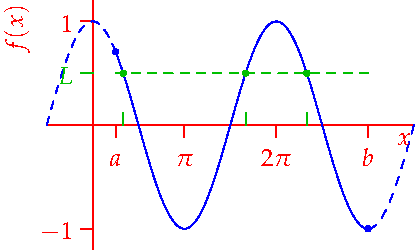
\includegraphics{intval2}
\end{example}



\begin{proof}
	Suppose WLOG that $f(a)<L<f(b)$ and let\par
	\begin{minipage}[t]{0.55\linewidth}\vspace{-15pt}
		\[
			\textcolor{Green}{S}=\{x\in[a,b]:f(x)<L\}
		\]
		Plainly $S\subseteq [a,b)$ is non-empty, hence $\xi:=\sup S$ exists and $\xi\in[a,b]$. It remains to show that $\xi$ satisfies the required properties.\medbreak
		
		By Exercise \ref{exs:extremevaluelemma}, $\exists(s_n)\subseteq S$ with $\lim s_n=\xi$.
		Since $f$ is continuous, $f(\xi)=\lim f(s_n)\le L$. In particular, $\xi\neq b$.
	\end{minipage}
	\hfill
	\begin{minipage}[t]{0.44\linewidth}\vspace{-15pt}
		\flushright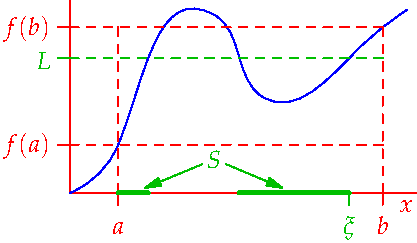
\includegraphics{intval}
	\end{minipage}
	\medbreak
	
	To finish, play a similar game with the sequence defined by $t_n=\min\{b,\xi+\frac 1n\}$ (see Exercise \ref{exs:ivtproof}).
\end{proof}


\begin{example}{}{}
	The intermediate value theorem is useful for demonstrating the existence of solutions to equations. For example, we show that the equation $x2^x=1$ has a solution.\par
	\begin{minipage}[t]{0.6\linewidth}\vspace{0pt}
		\begin{itemize}\itemsep2pt
			\item Observe that $g(x)=x2^x-1$ is continuous.
			\item $g(0)=-1<0$.
			\item $g(1)=1>0$.
			\item By the intermediate value theorem $\exists \xi\in(0,1)$ such that $g(\xi)=0$: that is $\xi\cdot 2^\xi=1$.
		\end{itemize}
	\end{minipage}
	\hfill
	\begin{minipage}[t]{0.39\linewidth}\vspace{-10pt}
		\flushright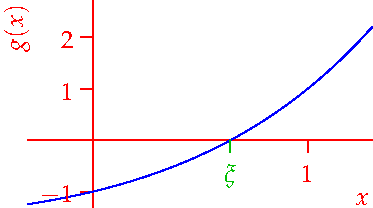
\includegraphics[scale=0.95]{intval3}
	\end{minipage}
	\bigbreak
	
	It is inefficient, but one can home in on $\xi$ by repeatedly halving the size of the interval: for instance,
	\[
		g(\tfrac 12)=\tfrac{\sqrt 2}2-1<0,\quad 
		g(\tfrac 34)=\tfrac 34\cdot 2^{3/4}-1\approx 0.26>0\ldots
		\implies \tfrac 12<\xi<\tfrac 34
	\]
\end{example}


\begin{cor}{}{}
	Continuous functions map intervals to intervals (or points).
\end{cor}

\begin{proof}
	An interval $I$ is characterized by the following property
	\[
		\forall x_1,x_2\in I,\ x\in\R,\ x_1<x<x_2\implies x\in I
	\]
	Let $f:I\to\R$ be continuous and suppose its range $f(I)$ is not a single point. If $f(a)<L<f(b)$, then $\exists \xi\text{ between $a,b$ such that }f(\xi)=L$. Otherwise said, $L\in f(I)$ and so $f(I)$ is an interval.
\end{proof}

More generally, if $\dom(f)=\bigcup I_n$ is written as a union of disjoint intervals and $f$ is continuous, then
\[
	\range(f)=\bigcup f(I_n)
\]
is also a union of intervals, though these need not be disjoint: a continuous function can bring intervals together, but cannot break them apart.\footnote{%
	More generally, if $f:U\to V$ is a continuous function between topological spaces and $a,b$ lie in the same \emph{component} of $U$, then $f(a),f(b)$ lie in the same component of $f(U)$. In our examples each component is an interval.}

\begin{example}{}{}
	The function $f(x)=\sqrt{x^2-4}$ has implied domain $(-\infty,-2]\cup[2,\infty)$ and range $[0,\infty)$. Both halves of the domain are mapped onto the same interval $\range(f)$ .
\end{example}

\goodbreak



\begin{exercises}
	\emph{Key concepts:\quad Extreme Value Theorem,\quad Intermediate Value Theorem}\vspace{-5pt}
	\begin{quote}
		\emph{Continuous functions preserve intervals}
	\end{quote}

	%\exstart Give examples of the following:\vspace{-5pt}
	\begin{enumerate}%\setcounter{enumi}{1}  
	  \item Give examples of the following:
	  \begin{enumerate}
	    \item An unbounded discontinuous function on a closed bounded interval.
	    \item An unbounded continuous function on a non-closed bounded interval.
	    \item A bounded continuous function on a closed unbounded interval which fails to attain its bounds.
		\end{enumerate}
		
	% 	\item Give an example of a discontinuous function on the interval $[0,1]$ which is not bounded. You may draw the function rather than provide a formula, provided it is clear what the function does.
	
	% 	\item Let $a<b$ be given to you. Give an example of a continuous function on $(a,b)$ which is unbounded. Give a second continuous function on $(a,b)$ which is bounded but does not attain its bounds.
		
		
		\item\label{exs:intvalinfty} Consider the function $f(x)=
		\begin{cases}
			x\sin\frac 1x&\text{if }x\neq 0\\
			0&\text{if }x=0
		\end{cases}$
		\begin{enumerate}
		  \item Explain why $f$ is continuous on any interval $I$.
		  \item Suppose $a<0<b$ and that $f(a),f(b)$ have opposite signs. If $L=0$, show that the intermediate value theorem is satisfied by \emph{infinitely many} distinct values $\xi$.
		\end{enumerate}

	
		\item Use the intermediate value theorem to prove that the equation $8x^3-12x^2-2x+1=0$ has at least 3 real solutions (and thus, by the fundamental theorem of algebra, exactly 3).
		
		
		\item\label{exs:ivtproof} Complete the proof of the intermediate value theorem by defining $t_n=\min(b,\xi+\frac 1n)$.
		
		
		\item\begin{enumerate}
		  \item Suppose $f:U\to\R$ is continuous and that $U=\bigcup\limits_{k=1}^nI_k$ is the union of a finite sequence $(I_k)$ of closed bounded intervals. Prove that $f$ is bounded and attains its bounds.
		  \item Let $U=\bigcup\limits_{n=1}^\infty I_n$, where $I_n=[\frac 1{2n},\frac 1{2n-1}]$ for each $n\in\N$. Give an example of a continuous function $f:U\to\R$ which is either unbounded or does not attain its bounds. Explain.
		\end{enumerate}
	\end{enumerate}
\end{exercises}


\clearpage


\subsection{Uniform Continuity}\label{sec:unifcont}

Recall Definition \ref{defn:cont}: $f:U\to\R$ is continuous at all points\footnote{%
	To promote symmetry, we use $y$ instead of $u$ for a generic point of $\dom(f)$.%
}
$y\in U$ provided
\[
	\forall y\in U,\ \forall\epsilon>0,\ \exists \delta>0\text{ such that }
	(\forall x\in U)\ \nm{x-y}<\delta
	\implies \nm{f(x)-f(y)}<\epsilon
\]
Note the order of the quantifiers: $\delta$ is permitted to depend \emph{both} on $y$ and $\epsilon$. In the naïve sense of continuity ($x$ close to $y\Longrightarrow f(x)$ close to $f(y)$), the meaning of \emph{close} can depend on the \emph{location} $y$. Uniform continuity is a stronger condition where the \textbf{meaning of \emph{close} is independent of location}.

\begin{defn}{}{}
	$f:U\to\R$ is \emph{uniformly continuous} if
	\[
		\forall\epsilon>0,\ \exists \delta>0\text{ such that }
		(\forall x,y\in U)\ \nm{x-y}<\delta
		\implies \nm{f(x)-f(y)}<\epsilon
	\]
\end{defn}
We've included the (typically) hidden quantifiers ($\forall x,y$) to make clear that $\delta$ is independent of $x,y$. Note also that the definition is now symmetric in $x,y$.


\begin{example}{}{unif1}
	Consider $f(x)=\frac 1x$.\par
	\begin{minipage}[t]{0.65\linewidth}\vspace{0pt}
		\begin{enumerate}
		\item If $0<a<b\le \infty$, then $f$ is uniformly continuous on $[a,b)$.\par
		Let $\epsilon>0$ be given and let $\delta=a^2\epsilon$. Then $\forall x,y\in[a,b)$,
		\[
			\nm{x-y}<\delta 
			\implies \nm{\frac 1x-\frac 1y} =\nm{\frac{y-x}{xy}}
			<\frac\delta{xy}\le\frac{\delta}{a^2}
			=\epsilon
		\]
		\item If $0<b\le\infty$, then $f$ is \emph{not} uniformly continuous on $(0,b)$.\smallbreak
		Let $\epsilon=1$ and suppose $\delta>0$ is given.\par
		Let $x=\min(\delta,1,\tfrac b2)$ and $y=\frac x2$.\par
		Certainly $x,y\in(0,b)$ and $\nm{x-y}=\frac x2\le\frac\delta 2<\delta$. However,
		\[
			\nm{f(x)-f(y)}=\frac 1x\ge 1=\epsilon
		\]
		\end{enumerate}
	\end{minipage}
	\hfill
	\begin{minipage}[t]{0.34\linewidth}\vspace{0pt}
		\flushright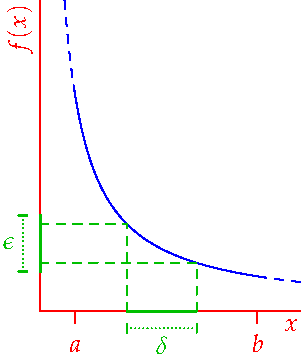
\includegraphics{unif1}
	\end{minipage}
	\bigbreak
	Think about how $\epsilon$ and $\delta$ must relate as one slides the intervals in the picture up/down and left/right.
\end{example}

Some intuition will help make sense of the example.
\begin{description}
	\item[Bounded/unbounded gradient] In part 1 $\epsilon=\delta{a^2}$, where $\frac 1{a^2}=\nm{f'(a)}$ bounds the gradient of $f$.\\
	By contrast, the slope of $f$ is \emph{unbounded} in part 2.
	\item[Extensibility] In part 1 the domain of $f$ may be extended to $a$ (and to $b$ if finite): $g:[a,b]\to\R:x\mapsto \frac 1x$ is continuous.
	In part 2, this is impossible: there is no continuous function $g:[0,b)\to\R$ such that $g(x)=\frac 1x$ whenever $x>0$.
\end{description}
Informally, if a continuous function $f$ has bounded gradient, or if you can `fill in the holes' at the endpoints of $\dom(f)$, then $f$ is uniformly continuous. When uniform continuity is used abstractly in a proof, it is often one of the above properties that is being invoked. The remainder of this section involves making these observations watertight.


\goodbreak


\begin{thm}{}{unifcontboundedslope}
	Let $f:I\to\R$ be continuous on an interval $I$ and differentiable with bounded derivative on the interior $I^\circ$. Then $f$ is uniformly continuous on $I$.
\end{thm}

The proof depends on the mean value theorem, which should be familiar from elementary calculus; we'll discuss a proof later on.

\begin{proof}
	Suppose $\nm{f'(x)}\le M$ on $I^\circ$. Let $\epsilon>0$ be given, let $\delta=\frac\epsilon M$ and suppose $(y,x)\subseteq I$. Then
	\begin{align*}
	\nm{x-y}<\delta&\implies \exists \xi\in I^\circ\text{ such that }f'(\xi)=\frac{f(x)-f(y)}{x-y} \tag{MVT}\\
	&\implies \nm{f(x)-f(y)}=\nm{f'(\xi)}\nm{x-y}<M\delta=\epsilon \tag*{\qedhere}
	\end{align*}
\end{proof}


Theorem \ref{thm:unifcontboundedslope} isn't a biconditional: for instance, Exercise \ref*{sec:unifcont}.\ref{exs:unifroots} shows that $f(x)=\sqrt x$ on $[0,\infty)$ and $g(x)=x^{1/3}$ on $\R$ are both uniformly continuous even though both have unbounded slope.\medbreak

We now discuss extensibility and how uniform continuity relates to continuity on closed sets. First we see that for closed bounded sets, uniform continuity is nothing new.

\begin{thm}{}{unifcontclosed}
	If $g:[a,b]\to\R$ is continuous, then it is uniformly continuous. 
\end{thm}

\begin{proof}
	Suppose $g$ is continuous but not uniformly so. Then
	\[
		\exists \epsilon>0\text{ such that }
		\forall\delta>0,\ \exists x,y\in [a,b]\text{ for which }
		\nm{x-y}<\delta\text{ and }
		\nm{g(x)-g(y)}\ge\epsilon \tag{$\ast$}
	\]
	For each $n\in\N$, let $\delta=\frac 1n$ to see that there exists sequences $(x_n),(y_n)\subseteq[a,b]$ satisfying the above.\\
	By Bolzano--Weierstraß, the bounded sequence $(x_n)$ has a convergent subsequence $x_{n_k}\to x\in[a,b]$. Clearly
	\[
		\nm{x_{n_k}-y_{n_k}}<\frac 1{n_k}\to 0\implies y_{n_k}\to x
	\]
	But then $\nm{g(x_{n_k})-g(y_{n_k})}\to 0$, which contradicts $(\ast)$.
\end{proof}

Now we build towards a partial converse.

\begin{lemm}{}{unifcont}
	If $f:U\to\R$ is uniformly continuous and $(x_n)\subseteq U$ is a Cauchy sequence, then $\bigl(f(x_n)\bigr)$ is also Cauchy.
\end{lemm}

\begin{proof}
	Let $\epsilon>0$ be given. Then:
	\begin{itemize}
	  \item (Uniform Continuity)\lstsp $\exists\delta>0$ such that $\nm{x-y}<\delta\Longrightarrow \nm{f(x)-f(y)}<\epsilon$.
	  \item (Cauchy)\lstsp $\exists N\in\N$ such that $m,n>N\Longrightarrow \nm{x_m-x_n}<\delta$.
	\end{itemize}
	Putting these together, we see that
	\[
		\exists N\in\N\text{ such that }m,n>N
		\implies \nm{f(x_m)-f(x_n)}<\epsilon
	\]
	Otherwise said, $\bigl(f(x_n)\bigr)$ is Cauchy.
\end{proof}
	
\goodbreak

We now see that a function $f:I\to \R$ is uniformly continuous on a bounded interval if and only it is has a \emph{continuous extension} $g:\cl I\to\R$ defined on the closure of its domain.

\begin{thm}{}{unifcontext}
	Suppose $f:I\to\R$ is continuous where $I$ is a bounded interval with endpoints $a<b$. Define $g:[a,b]\to\R$ via
	\[
		g(x)=
		\begin{cases}
	  	f(x)&\text{if }x\in I\\
	  	\lim f(x_n)&\text{whenever }(x_n)\subseteq I\text{ and }x_n\to a\\
	  	\lim f(x_n)&\text{whenever }(x_n)\subseteq I\text{ and }x_n\to b
	  \end{cases}
	 \]
	 Then $f$ is uniformly continuous if and only $g$ is well-defined ($g$ is continuous, \emph{if} well-defined).
\end{thm}

\begin{proof}
	\begin{description}
	\item[\normalfont ($\Rightarrow$)] Suppose $f$ is uniformly continuous on $I$ and that $a\not\in I$. Let $(x_n),(y_n)\subseteq I$ be sequences converging to $a$. To show that $g$ is well-defined, we must prove that $\bigl(f(x_n)\bigr)$ and $\bigl(f(y_n)\bigr)$ are convergent, and to the same limit. For this, we define a sequence
	\[
		(u_n)=(x_1,y_1,x_2,y_2,x_3,y_3,\ldots)
	\]
	Since $(x_n)$ and $(y_n)$ have the same limit $a$, we conclude that $u_n\to a$. But then $(u_n)$ is Cauchy. By Lemma \ref{lemm:unifcont}, $\bigl(f(u_n)\bigr)$ is also Cauchy and thus convergent. Since $\bigl(f(x_n)\bigr)$ and $\bigl(f(y_n)\bigr)$ are subsequences of a convergent sequence, they must also converge to the same (finite) limit.\par
	The argument when $b\not\in I$ is identical.
	\item[\normalfont ($\Leftarrow$)] If $g$ is well-defined then it is continuous (Definition \ref{defn:cont}, part 1); by Theorem \ref{thm:unifcontclosed} it is uniformly so. Since $f=g$ on a subset of $\dom(g)$, the same choice of $\delta$ will work for $f$ as for $g$: $f$ is therefore uniformly continuous.\qedhere
	\end{description}
\end{proof}


\begin{examples}{}{}
	\exstart Consider $f:x\mapsto x^2$. 
	\begin{enumerate}\setcounter{enumi}{1}
	  \item[]\begin{enumerate}
	    \item If $\dom(f)$ is the open interval $(-3,10)$, then $f$ is uniformly continuous since its derivative $f'(x)=2x$ is bounded ($\nm{f'(x)}\le 20$). The continuous extension is $g(x)=x^2$ on $[-3,10]$.
	    \item	If $\dom(f)$ is the infinite interval $(-3,\infty)$, then neither Theorem \ref{thm:unifcontboundedslope} nor \ref{thm:unifcontext} applies: both $f'$ and the domain $(-3,\infty)$ are unbounded.\par
			Instead, note that if $\epsilon=1$, then for any $\delta>0$, we can choose $x=\frac 1\delta$ and $y=\frac 1\delta+\frac\delta 2$. Clearly
			\[
				\nm{x-y}=\frac\delta 2<\delta\text{ and }
				\nm{x^2-y^2}=1+\frac{\delta^2}4>1=\epsilon
			\]
			whence $f$ is not uniformly continuous.
	  \end{enumerate}
		\item $f(x)=x\sin \frac 1x$ is continuous on the interval $(0,\infty)$. Strictly, neither Theorem \ref{thm:unifcontboundedslope} nor \ref{thm:unifcontext} apply since the derivative
		\[
			f'(x)=\sin\frac 1x-\frac 1x\cos\frac 1x
		\]
		is unbounded as is the domain. However, by breaking the domain into two pieces\ldots 
		\begin{itemize}
		  \item On $[1,\infty)$, the derivative is bounded: $\nm{f'(x)}\le 1+\frac 1{x^2}\le 2$ by the triangle inequality. Theorem \ref{thm:unifcontboundedslope} says $f$ is uniformly continuous on $[1,\infty)$.
		  \item $f$ is continuous on $(0,1]$ and, by the squeeze theorem
		  \[
		  	x_n\to 0^+\implies \lim f(x_n)=0
		  \]
		  Extending $f$ so that $f(0)=0$ defines a continuous extension. By Theorem \ref{thm:unifcontext}, $f$ is uniformly continuous on $(0,1]$.
	 	\end{itemize}
	 	Putting this together (Exercise \ref{exs:unifcontunion}), $f$ is uniformly continuous on $(0,\infty)$. Indeed the function
	 	\[
	 		h(x)=
	 		\begin{cases}
	 			x\sin\frac 1x&\text{if }x\neq 0\\
	 			0&\text{if }x=0
	 		\end{cases}
	 	\]
	 	is uniformly continuous on $\R$.
	\end{enumerate}
\end{examples}


\begin{exercises}
	\emph{Key concepts:\quad Uniform Continuity (same $\delta$ for all locations),\quad Bounded gradient,}\vspace{-5pt}
	\begin{quote}
		\emph{Continuous extensions}
	\end{quote}
	
	%\exstart Which functions are uniformly continuous? Justify your answers.\vspace{-5pt}
	\begin{enumerate}\setcounter{enumi}{1}  
	  \item Which functions are uniformly continuous? Justify your answers.
	  \begin{enumerate}
	    \item \makebox[200pt][l]{$f(x)=x^4$ on $[-1,1]$\hfill (b) }
	    $f(x)=x^4$ on $(-1,1]$
	    \setcounter{enumii}{2}
	    \item \makebox[200pt][l]{$f(x)=x^{-4}$ on $(0,2]$\hfill (d) }
	    $f(x)=x^{-4}$ on $(1,2]$
	    \setcounter{enumii}{4}
	    \item $f(x)=x^2\sin\frac 1x$ on $(0,1]$
	  \end{enumerate}
	  
	  
	  \item Prove that each function is uniformly continuous by verifying the $\epsilon$--$\delta$ property.
	  \begin{enumerate}
	    \item \makebox[200pt][l]{$f(x)=2x-14$ on $\R$\hfill (b) }
	    $f(x)=x^3$ on $[1,5]$
	    \setcounter{enumii}{2}
	    \item \makebox[200pt][l]{$f(x)=x^{-1}$ on $(1,\infty)$\hfill (d) }
	    $f(x)=\frac{x+1}{x+2}$ on $[0,1]$
	  \end{enumerate}
	  
	  
	  \item Prove that $f(x)=x^4$ is not uniformly continuous on $\R$.
	  
	  
	  \item\begin{enumerate}
	     \item Suppose $f$ is uniformly continuous on a bounded interval $I$. Prove that $f$ is bounded on $I$.
	     \item Use part (a) to write down a bounded interval on which the function $f(x)=\tan x$ is defined, but \emph{not} uniformly continuous.
	  \end{enumerate}
	
	
	  \item\label{exs:unifroots} Both parts of this question are easy using Exercise \ref{exs:unifcontunion}. Do them explicitly using the $\epsilon$--$\delta$ property.
	  \begin{enumerate}
	    \item Let $f(x)=\sqrt x$ with domain $[0,\infty)$. Show that $f'(x)$ is unbounded, but that $f$ is still uniformly continuous on $[0,\infty)$.\par
	    (\emph{Hint: let $\delta=(\frac\epsilon 2)^3$ and consider the cases $x\ge y\ge 0$, $x\le y\le 0$ and $x>0>y$ separately})
	    \item Prove that $g(x)=x^{1/3}$ is uniformly continuous on $\R$.\par
	    (\emph{Hint: let $\delta=\epsilon^2$ and WLOG assume $0\le y\le x$. Now compute $(\sqrt y+\epsilon)^2$\ldots })
	  \end{enumerate}


		\item\label{exs:unifcontunion} Suppose $f$ is uniformly continuous on intervals $U_1,U_2$ for which $U_1\cap U_2$ is non-empty. Prove that $f$ is uniformly continuous on $U_1\cup U_2$.\par
		(\emph{Hint: if $x,y$ do not lie in the same $U_1,U_2$, choose some $a\in U_1\cap U_2$ between $x$ and $y$})
		
	\end{enumerate}
\end{exercises}
\vfil
\goodbreak



\setcounter{subsection}{19}
\subsection{Limits of Functions}

In elementary calculus you likely saw many calculations of the following form:
\[
	\lim_{x\to 3}\frac{x^2-9}{x-3}
	=\lim_{x\to 3}\frac{(x-3)(x+3)}{x-3}
	=\lim_{x\to 3}(x+3)=6
\]
Loosely speaking, this means that if $(x_n)\subseteq\R\setminus\{3\}$ is a sequence converging to 3, then $\bigl(f(x_n)\bigr)$ converges to 6. Our goal in this section is to make this notation precise.

\begin{defn}{}{leftrightlimit}
	Suppose $f:U\to\R$, that $S\subseteq U$, and that $a$ is the limit of some sequence in $S$.\smallbreak
	We say that $L$ is the \emph{limit of $f(x)$ as $x$ tends to $a$ along $S$,}  written $\smash{\lim\limits_{x\to a^S}f(x)=L}$, provided 
	\[
		\forall (x_n)\subseteq S,\ \lim x_n=a\implies \lim f(x_n)=L
	\]
	We can now define one-sided and two-sided limits of functions:
	\begin{description}\itemsep2pt
		\item[\normalfont\emph{Right-hand limit}:] $\lim\limits_{x\to a^+}f(x)=L$ means $\exists S=(a,b)\subseteq U$ for which $\lim\limits_{x\to a^S}f(x)=L$
		\item[\normalfont\emph{Left-hand limit}:] $\lim\limits_{x\to a^-}f(x)=L$ means $\exists S=(c,a)\subseteq U$ for which $\lim\limits_{x\to a^S}f(x)=L$
		\item[\normalfont\emph{Two-sided limit}:] $\lim\limits_{x\to a}f(x)=L$ means $\exists S=(c,a)\cup(a,b)\subseteq U$ for which $\lim\limits_{x\to a^S}f(x)=L$
	\end{description}
\end{defn}

\vfil

\begin{itemize}
  \item If $U=\dom(f)$ is unbounded, then the one-sided definitions apply when $a=\pm\infty$. We omit the $\pm$ modifiers: for instance,
  \[
  	\lim_{x\to\infty}f(x)=L\iff 
  	\lim\limits_{x\to\infty^S}f(x)=L\text{ for some }
  	S=(c,\infty)\subseteq U
  \]
	\item\label{it:contlimit} Note that $f$ need not be defined at $a$, though $U=\dom(f)$ must contain at least some \emph{punctured neighborhood} of $a$ (one-sided for a one-sided limit). This will certainly happen if $U$ is a union of intervals of positive length. In such a case, one may simply replace $S$ with $U\setminus\{a\}$ in the definition: this is precisely what we did in the motivating example where $U=\R\setminus\{3\}$.\par
%   \[
%   	\lim\limits_{x\to a^{(\pm)}}f(x)=L\iff
%   	\Bigl(\forall (x_n)\subseteq U\setminus\{a\},\  \lim x_n=a
%   	\implies \lim f(x_n)=L\Bigr)
%   \]
  Moreover, in such a situation, Definition \ref{defn:cont} recovers a familiar idea from elementary calculus:
  \[
  	f \text{ is continuous at } a\in U
  	\iff f(a)=
  	\begin{cases}
  		\lim\limits_{x\to a} f(x)&\text{when }a\in U^\circ\\
  		\lim\limits_{x\to a^\pm} f(x)&\text{when }a\in U\setminus\partial U
  	\end{cases}
  	\tag{$\ast$}
 	\]
 	Warning! When $\dom(f)$ does not contain a punctured neighborhood of $a$, the right hand side doesn't exist and the assertion is \emph{false}!
  \item By modifying the proof of Theorem \ref{thm:contdefequiv} when $a,L\in\R$ are finite, we can restate using $\epsilon$-language. For instance, $\lim\limits_{x\to a}f(x)=L$ means
  \[
  	\forall\epsilon>0,\ \exists \delta>0\text{ such that }(\forall x\in\R)\ 0<\nm{x-a}<\delta\implies \nm{f(x)-L}<\epsilon
  \]
  If $a$ and/or $L$ is infinite, use the language of unboundedness: e.g. $\lim\limits_{x\to a}f(x)=\infty$ means
  \[
  	\forall M>0,\ \exists \delta>0\text{ such that }0<\nm{x-a}<\delta\implies f(x)>M
  \]
  There are \emph{fifteen} distinct combinations: \emph{three} two-sided and \emph{six} each of the one-sided limits!
\end{itemize}
\goodbreak


\begin{examples}{}{}
	\exstart Let $f(x)=\frac{2+x}x$ where $\dom(f)=U=\R\setminus\{0\}=(-\infty,0)\cup(0,\infty)$
	\begin{enumerate}\setcounter{enumi}{1}
	  \item[]	The following should be clear:
		\[
			\lim\limits_{x\to 3}f(x)=\frac 53\qquad 
			\lim\limits_{x\to \infty}f(x)=1
		\]
		To compute the first, for instance, we could choose $S=(0,3)\cup(3,\infty)$; if $(x_n)\subseteq S$ and $x_n\to 3$, then the limit laws justify the first claim
		\[
			\lim_{n\to\infty}f(x_n)=\frac{2+3}{3}=\frac 53
		\]
		as does the fact that $f$ is continuous at $x=3$. The second claim can be checked similarly.\smallbreak
		\begin{minipage}[t]{0.6\linewidth}\vspace{0pt}
		We can take one-sided limits at $x=0$:
		\[
			\lim\limits_{x\to 0^+}f(x)=\infty
			\quad\text{and}\quad
			\lim\limits_{x\to 0^-}f(x)=-\infty
		\]
		For instance, let $(x_n)\subseteq (0,\infty)$ satisfy $x_n\to 0$. Again, the limit laws show that $\lim\limits_{n\to\infty}f(x_n)=\infty$, which is enough to justify the first claim.\medbreak
		Finally, the sequences defined by $x_n=\frac 1n$ and $y_n=-\frac 1n$ both lie in $S=\R\setminus\{0\}$ and converge to zero, yet
		\[
			\lim_{n\to\infty} f(x_n)=\infty
			\neq -\infty =\lim_{n\to\infty} f(y_n)
		\]
		It follows that the two-sided limit $\displaystyle\lim\limits_{x\to 0}f(x)$ does not exist.
	\end{minipage}
	\hfill
	\begin{minipage}[t]{0.39\linewidth}\vspace{0pt}
		\flushright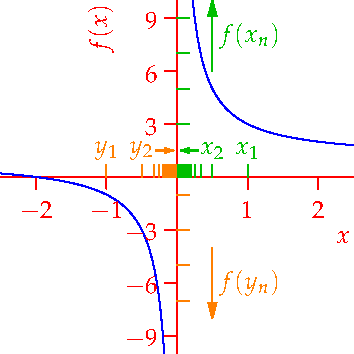
\includegraphics{limitex2}
	\end{minipage}
		
	\item Let $f(x)=\frac 1{x^2}$ whenever $x\neq 0$ and additionally let $f(0)=0$. Here the two-sided limit exists
	\[
		\lim_{x\to 0}f(x)=\infty
	\]
	However the value of the function at $x=0$ does not equal this limit: clearly $f$ is discontinuous at $x=0$.
		
	\item We revisit our motivating example. Let $f(x)=\frac{x^2-9}{x-3}$ have domain $U=\R\setminus\{3\}$. Whenever $x_n\neq 3$, we see that
	\[
		f(x_n)=\frac{(x_n-3)(x_n+3)}{x_n-3}=x_n+3
	\]
	By the limit laws, we conclude that $\lim f(x_n)=3+3=6$ and so
	\[
		\lim\limits_{x\to 3}\frac{x^2-9}{x-3}=6
	\]
	%	Implicit in the original calculation is that the function $f$ has domain \emph{excluding} 3. Indeed the original calculation relies on the following updating of the limit laws to our new context.
	\end{enumerate}
\end{examples}

\vfil
\goodbreak

Since we referenced the limit laws for sequences so often in the examples, it is appropriate to update them to this new context. We do so without proof.

\begin{cor}{Limit Laws for functions}{}
	Suppose $f,g:U\to\R$ satisfy $L=\lim\limits_{x\to a}f(x)$ and $M=\lim\limits_{x\to a}g(x)$ exist. Then,
	\begin{enumerate}
	  \item $\displaystyle\lim_{x\to a}(f+g)(x)=L+M$.
	  \item $\displaystyle\lim_{x\to a}(fg)(x)=LM$.
	  \item $\displaystyle\lim_{x\to a}\left(\frac fg\right)(x)=\frac LM$\quad (requires $M\neq 0$).
		\item If $L\in\R$ and $h$ is continuous at $L$, then $\displaystyle\lim\limits_{x\to a}(h\circ f)(x)=h(L)$.
		\item (Squeeze Theorem)\ If $L=M$ and $f(x)\le h(x)\le g(x)$ for all $x\in U$, then $\lim\limits_{x\to a}h(x)=L$.
	\end{enumerate}
	The corresponding results for one-sided limits also hold.
\end{cor}

As with the original limit laws for sequences, parts 1--3 apply provided the limits are not \emph{indeterminate forms} (e.g.\ $\infty-\infty$, $0\cdot\infty$, $\frac 00$, $\frac\infty\infty$). We'll see later how l'Hôpital's rule may be applied to such cases.


\begin{examples}{}{}
	\exstart Since $f(x)=\frac{x^2+5}{3x^2-2}$ is a rational function (continuous at all points of its domain), we quickly conclude that
	\[
		\lim\limits_{x\to 2}\frac{x^2+5}{3x^2-2}=f(2)=\frac 9{10}
	\]
	Alternatively, we may tediously invoke the other parts of the theorem:
	\begin{align*}
		\lim\limits_{x\to 2}\frac{x^2+5}{3x^2-2}
		&\overset{(3)}{=} \frac{\lim(x^2+5)}{\lim(3x^2-2)} \overset{(1)}{=} 
		\frac{\lim x^2+\lim 5}{\lim 3x^2-\lim 2} \overset{(2)}{=} 
		\frac{(\lim x)^2+5}{(\lim 3)(\lim x)^2-2}\\
		&=\frac{2^2+5}{3\cdot 2^2-2} =\frac 9{10}
	\end{align*}
	\begin{enumerate}\setcounter{enumi}{1}
		\item As $x\to\infty$, the simplistic approach results in a nonsense indeterminate form:
		\[
			\lim_{x\to\infty}\frac{x^2+5}{3x^2-2} \overset{\text{?}}{=} 
			\frac{\lim(x^2+5)}{\lim(3x^2-2)} \overset{\text{?}}{=} 
			\frac\infty\infty
		\]
		However, a little pre-theorem algebra quickly yields\footnotemark
		\[
			\lim_{x\to\infty}\frac{x^2+5}{3x^2-2} 
			=\lim_{x\to\infty}\frac{1+5x^{-2}}{3-2x^{-2}} 
			=\frac{\lim(1+5x^{-2})}{\lim(3-2x^{-2})} 
			=\frac 13
		\]
	\end{enumerate}
\end{examples}

\footnotetext{%
	Be careful! The expressions $\frac{x^2+5}{3x^2-2}$ and $\frac{1+5x^{-2}}{3-2x^{-2}}$ do not describe the same function, yet their \emph{limits} at $\infty$ are equal. The ease of equating these limits is one of the advantages of the `$\exists S$' formulation in Definition \ref{defn:leftrightlimit}. Think about why; what is a suitable set $S$ in this context?%
}

\vfil

\goodbreak


\boldsubsubsection{Classification of Discontinuities}

We now consider the ways in which a function can fail to be continuous.

\begin{defn}{}{}
	Suppose that a function is continuous on an interval except at finitely many values: we call these \emph{isolated discontinuities.}
\end{defn}

\begin{examples}{}{}
	\exstart $f(x)=\frac 1x$ has a discontinuity at $x=0$ since it is continuous on the interval $\R$, except at one point $x=0$. Note that a function need not be defined at a discontinuity!
	\begin{enumerate}\setcounter{enumi}{1}
	  \item $f(x)=\frac 1{\sin \frac 1x}$ has a \emph{non-isolated discontinuity} at $x=0$: on any interval containing zero, $f$ has infinitely many discontinuities: $x=\frac 1{\pi n}$ where $\nm n\in\N$.
	\end{enumerate}
\end{examples}


The next result helps us classify isolated discontinuities.

\begin{thm}{}{sidedlimitsequal}
	Let $f:U\to\R$ and suppose $a\in U^\circ$ is an interior point. Then
	\[
		\lim\limits_{x\to a}f(x)=L \iff \lim\limits_{x\to a^+}f(x)=L=\lim\limits_{x\to a^-}f(x)
	\]
\end{thm}

\begin{proof}
	\begin{description}
	\item[\normalfont ($\Rightarrow$)] Let $S=(c,a)\cup(a,b)$ satisfy the definition for $\lim\limits_{x\to a}f(x)=L$. Since any sequence (say) in $S^+$ is also in $S$, plainly $S^+=(a,b)$ and $S^-=(c,a)$ satisfy the one-sided definitions.
	\item[\normalfont ($\Leftarrow$)] Suppose $S^-=(c,a)$ and $S^+=(a,b)$ satisfy the one-sided definitions and denote $S=S^-\cup S^+$. Let $(x_n)\subseteq S$ be such that $x_n\to a$. Clearly $(x_n)$ is the disjoint union of two subsequences $(x_n)\cap S^+$ and $(x_n)\cap S^-$, both of which\footnotemark converge to $a$. There are three cases:%\vspace{-5pt}
	\begin{description}\itemsep0pt
		\item[$L$ \normalfont{finite}:] Let $\epsilon>0$ be given. Because of the one-sided limits,
		\begin{itemize}
	  	\item $\exists N_1$ such that $n>N_1$ and $x_n>a\implies \nm{f(x_n)-L}<\epsilon$
	  	\item $\exists N_2$ such that $n>N_2$ and $x_n<a\implies \nm{f(x_n)-L}<\epsilon$
		\end{itemize}
		Now let $N=\max(N_1,N_2)$ in the definition of limit to see that $\lim f(x_n)=L$. Since this holds for all sequences $(x_n)\subseteq S$ converging to $a$, we conclude that $\lim\limits_{x\to a}f(x)=L$.
		\item[$L=\pm\infty$:] This is an exercise.\hfill\qedhere
	
	% 	\item[$L=\infty$:] Let $M>0$ be given and repeat the above to see that $\lim f(x_n)=\infty$: the only required modification is to replace $\nm{f(x_n)-L}<\epsilon$ by $f(x)>M$,
	% 	\item[$L=-\infty$:] This is almost identical to the previous case.\hfill\qedhere
		\end{description}
	\end{description}
\end{proof}

\footnotetext{%
	It is possible for \emph{one} of these subsequences to be finite; say if $x_n>a$ for all large $n$. This is of no concern; one of the $\epsilon$-$N$ conditions would be empty and thus vacuously true.%
}


\begin{example}{}{}
	Recalling elementary calculus, we show that the following is continuous at $x=1$:
	\[
		f(x)=
		\begin{cases}
			x^2-3&\text{if }x\ge 1\\
			3-5x&\text{if }x<1
		\end{cases}
	\]
	\begin{description}
	  \item[\normalfont\emph{Step 1}:] Compute the left- and right-handed limits and check that these are equal:
	  \[
	  	\lim\limits_{x\to 1^-}f(x)=\lim\limits_{x\to 1^-}3-5x=-2,\qquad  
	  	\lim\limits_{x\to 1^+}f(x)=\lim\limits_{x\to 1^+}x^2-3=-2
	  \]
	  \item[\normalfont\emph{Step 2}:] Check that the value of the limits equals that of the function: $f(1)=1^2-3=-2$.
	\end{description}
\end{example}

\goodbreak


Recalling $(\ast)$ on page \pageref{it:contlimit}, we describe the different types of isolated discontinuity at some point $a$.
\begin{description}
	\begin{minipage}[t]{0.65\linewidth}\vspace{0pt}
	\item[Removable discontinuity] The two-sided limit $\lim\limits_{x\to a}f(x)=L$ is finite, and either:
	\begin{quote}
	  $f(a)\neq L$ or $f(a)$ is undefined.
	\end{quote}
	The term comes from the fact that we can remove the discontinuity by changing the behavior of $f$ only at $x=a$:
	\[
		\tilde f(x):=
		\begin{cases}
			f(x)&\text{if }x\neq a\\
			\lim\limits_{x\to a}f(x)&\text{if }x=a
		\end{cases}
	\]
	is now continuous at $x=a$. In the pictures,
	\[
		f_1(x)=\frac{x^2-9}{x-3}
		\quad\text{and}\quad 
		f_2(x)=
		\begin{cases}
  		x\sin(\frac 1x)&\text{if }x\neq 0\\
  		1&\text{if }x=0
  	\end{cases}
  \]
	have removable discontinuities at $x=3$ and $0$ respectively.
	\end{minipage}
	\hfill
	\begin{minipage}[t]{0.34\linewidth}\vspace{0pt}
		\flushright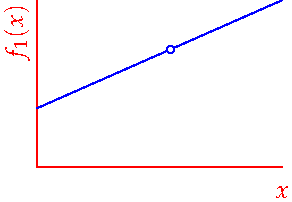
\includegraphics{discont1}\\\vfill
		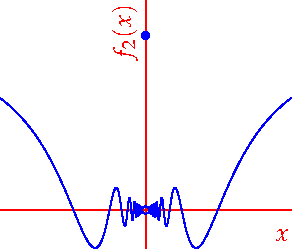
\includegraphics{discont2}
	\end{minipage}
	\smallbreak
	\begin{minipage}[t]{0.65\linewidth}\vspace{0pt}
		\item[Jump Discontinuity] The one-sided limits are finite but \emph{not equal.} A jump discontinuity cannot be removed by changing or inserting a value at $x=a$. The picture shows
		\[
			g(x)=\frac{\nm x}x=
			\begin{cases}
				1&\text{if }x>0\\
				-1&\text{if }x<0
			\end{cases}
		\]
		with a jump discontinuity at $x=0$.
	\end{minipage}
	\hfill
	\begin{minipage}[t]{0.34\linewidth}\vspace{0pt}
		\flushright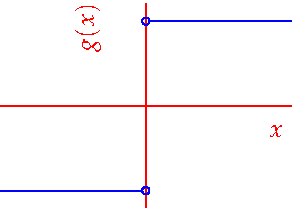
\includegraphics{discont3}
	\end{minipage}
	\smallbreak
	\begin{minipage}[t]{0.65\linewidth}\vspace{0pt}
		\item[Infinite discontinuity] The one-sided limits exist but at least one is infinite. We call the line $x=a$ a  \emph{vertical asymptote.} The picture shows
		\[
			h(x)=\frac 1{x^2}
		\]
		with an infinite discontinuity $x=0$. The fact that the one-sided limits of $h$ are equal (and infinite) is irrelevant.
	\end{minipage}
	\hfill
	\begin{minipage}[t]{0.34\linewidth}\vspace{0pt}
		\flushright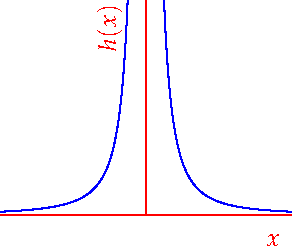
\includegraphics{discont4}
	\end{minipage}
	\smallbreak
	\begin{minipage}[t]{0.65\linewidth}\vspace{0pt}
		\item[Essential discontinuity] At least one of the one-sided limits does not exist. The picture shows $j(x)=\sin\frac 1x$ for which neither of the limits $\lim\limits_{x\to 0^\pm}j(x)$ exist.
	\end{minipage}
	\hfill
	\begin{minipage}[t]{0.34\linewidth}\vspace{0pt}
		\flushright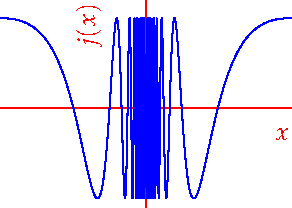
\includegraphics{discont5}
	\end{minipage}
\end{description}
It is also reasonable to refer to removable, infinite or essential discontinuities at interval endpoints.

\clearpage

\begin{exercises}
	\emph{Key concepts:\quad $\lim\limits_{x\to a}f(x)=L$,\quad $\epsilon,\delta,M,N$  versions,\quad Limit Laws,\quad Discontinuities}


	%\exstart For the function $f(x)=\frac{x^3}{\nm x}$, determine the limits $\lim\limits_{x\to\infty}f(x)$, $\lim\limits_{x\to-\infty}f(x)$, $\lim\limits_{x\to 0^-}f(x)$, $\lim\limits_{x\to 0^+}f(x)$ and $\lim\limits_{x\to 0}f(x)$, if they exist.
	
	\begin{enumerate}\itemsep0pt%\setcounter{enumi}{1}\itemsep0pt 
	  \item Given $f(x)=\frac{x^3}{\nm x}$, find $\lim\limits_{x\to\infty}f(x)$, $\lim\limits_{x\to-\infty}f(x)$, $\lim\limits_{x\to 0^-}f(x)$, $\lim\limits_{x\to 0^+}f(x)$ and $\lim\limits_{x\to 0}f(x)$, if they exist.
	  
	  \item Evaluate the following limits \emph{using the methods of this section}
	  \begin{enumerate}
	    \item \makebox[140pt][l]{$\displaystyle\lim_{x\to a}\frac{\sqrt x -\sqrt a}{x-a}$\hfill(b)}
	    \space$\displaystyle\lim_{x\to a}\frac{x^{-3/2}-a^{-3/2}}{x-a}$
	    \item[(c)] \makebox[140pt][l]{$\displaystyle\lim\limits_{x\to 0}\frac{\sqrt{1+3x^2}-1}{x^2}$\hfill(d)}
	    \space $\displaystyle\lim\limits_{x\to -\infty}\frac{\sqrt{4+3x^2}-2}{x}$
	  \end{enumerate}
	  
	 	%\item Evaluate the limits $\textstyle\lim\limits_{x\to 0}\frac{\sqrt{1+3x^2}-1}{x^2}$. Justify all your steps.
	  
	  \item Suppose that the limits $L=\lim\limits_{x\to a^+}f(x)$ and $M=\lim\limits_{x\to a^+}g(x)$ exist.
	  \begin{enumerate}
	    \item Suppose $f(x)\le g(x)$ for all $x$ in some interval $(a,b)$. Prove that $L\le M$.
	    \item Do we have the same conclusion if we have $f(x)<g(x)$ on $(a,b)$, or can we conclude that $L<M$? Prove your assertion, or give a counter-example.
	  \end{enumerate}
	  
	  
	  \item Suppose that $\lim\limits_{x\to\infty}f(x)=\lim\limits_{x\to\infty}g(x)=\infty$. Using \emph{only} this information, which of the following can you evaluate? Prove your assertions in each case.
	  \begin{enumerate}
	    \item $\lim\limits_{x\to\infty}(f+g)(x)$\qquad
			(b) \ $\lim\limits_{x\to\infty}(f-g)(x)$\qquad
			(c) \ $\lim\limits_{x\to\infty}(fg)(x)$\qquad
			(d) \ $\lim\limits_{x\to\infty}(f/g)(x)$
	  \end{enumerate}
	  
	  
	  \item Complete the proof of Theorem \ref{thm:sidedlimitsequal} by considering the $L=\pm\infty$ cases.
	  
	  
	  \item Graph $f:\R\to\R$, find and identify the types of its discontinuities.
	  \[
	  	f(x)=
	  	\begin{cases}
	    	0&x=0,\pm 1\\
	      \frac x{\nm x}&0<\nm x<1\\
	      x^2&\nm x>1
	    \end{cases}
	  \]
	  
	  
	  \item Find the discontinuities and identify their types for the following function
	  \[
	  	f(x)=
	  	\begin{cases}
	  		\frac 1x\sin\frac 1x&\text{if $x<0$ or $x>1$}\\
	  		\frac 1x&\text{if }0<x\le 1
	  	\end{cases}
	  \]
	  
	  
	  \item Let $a\in U^\circ$. Verify the claim following Definition \ref{defn:leftrightlimit}: $\lim\limits_{x\to a}f(x)=L$ if and only if
	  \[
	  	\forall\epsilon>0,\exists\delta>0\text{ such that }0<\nm{x-a}<\delta\implies \nm{f(x)-L}<\epsilon
	  \]
	  
	  
	  \item Recall Exercise \ref*{sec:cont}.\ref{exs:isolatedcont}, where we saw that a function $f:U\to\R$ is continuous at any isolated point $a\in U$.
	  \begin{enumerate}
	    \item Any function with domain $\dom(f)=\Z$ is continuous everywhere! Explain why we cannot define any limits $\lim\limits_{x\to a^{(\pm)}}f(x)$ for such a function.\par
	    (\emph{Hint: Being unable to define a limit is different from saying $\lim f(x)=\text{DNE}$: see page \pageref{it:contlimit}.})
	    \item Suppose $g(x)=x^2h(x)$ has $\dom(g)=\{0\}\cup\{\tfrac 1n:n\in\Z\}$, where $h$ is any function taking values in the interval $[-1,1]$. Explain why $g$ is continuous at every point of its domain.
		\end{enumerate}
		(\emph{These awkward examples of continuity can be avoided if we follow our usual approach where a domain is a union of intervals of positive length. This restriction is essentially baked in to the Definition \ref{defn:leftrightlimit}.})
	  
	\end{enumerate}
\end{exercises}